%%%%%%%%%%%%%%%%%%%%%%%%%%%%%%%%%%%%%%%%%
% Jacobs Landscape Poster
% LaTeX Template
% Version 1.0 (29/03/13)
%
% Created by:
% Computational Physics and Biophysics Group, Jacobs University
% https://teamwork.jacobs-university.de:8443/confluence/display/CoPandBiG/LaTeX+Poster
% 
% Further modified by:
% Nathaniel Johnston (nathaniel@njohnston.ca)
%
% This template has been downloaded from:
% http://www.LaTeXTemplates.com
%
% License:
% CC BY-NC-SA 3.0 (http://creativecommons.org/licenses/by-nc-sa/3.0/)
%
%%%%%%%%%%%%%%%%%%%%%%%%%%%%%%%%%%%%%%%%%

%----------------------------------------------------------------------------------------
%	PACKAGES AND OTHER DOCUMENT CONFIGURATIONS
%----------------------------------------------------------------------------------------

\documentclass[final]{beamer}

\usepackage[scale=1.24]{beamerposter} % Use the beamerposter package for laying out the poster
\usepackage[version=4]{mhchem}
\usetheme{confposter} % Use the confposter theme supplied with this template

\setbeamercolor{block title}{fg=ngreen,bg=white} % Colors of the block titles
\setbeamercolor{block body}{fg=black,bg=white} % Colors of the body of blocks
\setbeamercolor{block alerted title}{fg=white,bg=dblue!70} % Colors of the highlighted block titles
\setbeamercolor{block alerted body}{fg=black,bg=dblue!10} % Colors of the body of highlighted blocks
% Many more colors are available for use in beamerthemeconfposter.sty

%-----------------------------------------------------------
% Define the column widths and overall poster size
% To set effective sepwid, onecolwid and twocolwid values, first choose how many columns you want and how much separation you want between columns
% In this template, the separation width chosen is 0.024 of the paper width and a 4-column layout
% onecolwid should therefore be (1-(# of columns+1)*sepwid)/# of columns e.g. (1-(4+1)*0.024)/4 = 0.22
% Set twocolwid to be (2*onecolwid)+sepwid = 0.464
% Set threecolwid to be (3*onecolwid)+2*sepwid = 0.708

\newlength{\sepwid}
\newlength{\onecolwid}
\newlength{\twocolwid}
\newlength{\threecolwid}
\setlength{\paperwidth}{48in} % A0 width: 46.8in
\setlength{\paperheight}{36in} % A0 height: 33.1in
\setlength{\sepwid}{0.024\paperwidth} % Separation width (white space) between columns
\setlength{\onecolwid}{0.22\paperwidth} % Width of one column
\setlength{\twocolwid}{0.464\paperwidth} % Width of two columns
\setlength{\threecolwid}{0.708\paperwidth} % Width of three columns
\setlength{\topmargin}{-0.5in} % Reduce the top margin size
%-----------------------------------------------------------

\usepackage{graphicx}  % Required for including images

\usepackage{booktabs} % Top and bottom rules for tables

%----------------------------------------------------------------------------------------
%	TITLE SECTION 
%----------------------------------------------------------------------------------------

\title{Genetic Sugar Factories: Engineering Cyanobacteria to Secrete Sucrose} % Poster title
\author{\textbf{K. Ledalla, L. Velikov,} P. Aggarwal, S. Budhan, D. Kwasniak, M. Lee, N. Lo, M. Mullin, L.Y. Pan, J. Rakhimov, R. Ruzic, W. Sea, M. Shah, S. Vincent} % Author(s)

\institute{Stony Brook University iGEM Team} % Institution(s)

%----------------------------------------------------------------------------------------

\begin{document}

\addtobeamertemplate{block end}{}{\vspace*{2ex}} % White space under blocks
\addtobeamertemplate{block alerted end}{}{\vspace*{2ex}} % White space under highlighted (alert) blocks

\setlength{\belowcaptionskip}{2ex} % White space under figures
\setlength\belowdisplayshortskip{2ex} % White space under equations

\begin{frame}[t] % The whole poster is enclosed in one beamer frame

\begin{columns}[t] % The whole poster consists of three major columns, the second of which is split into two columns twice - the [t] option aligns each column's content to the top

\begin{column}{\sepwid}\end{column} % Empty spacer column

\begin{column}{\onecolwid} % The first column

%----------------------------------------------------------------------------------------
%	INTRODUCTION
%----------------------------------------------------------------------------------------

\begin{block}{Introduction}

The research question, put simply, is: can we genetically engineer cyanobacteria (in our case, \textit{Synechococcus elongatus} PCC 7942) to secrete sucrose?

\begin{center}
\textit{Current Findings}
\end{center}

\begin{itemize}
\item Scientists successfully engineered S. elongatus to secrete sucrose in large quantities, but process not commercialized because of high harvesting costs and inefficient photobioreactor design \cite{Qiao:2017jd}
\item Photosynthetic cyanobacteria like S. elongatus PCC 7942 produce sucrose more efficiently than both corn and sugarcane, fixing carbon dioxide (\ce{CO2}) and secreting roughly 80\% of fixed carbon as sucrose without the need for cell-harvesting \cite{Ducat:2012jd}
\item Our project goal to make cyanobacteria carbon sequestration industrially viable
\end{itemize}

\begin{center}
\textit{Why?}
\end{center}

\begin{itemize}
\item Crops like corn and sugarcane only allocate 20\% of fixed carbon as sucrose, and large amounts of land and fertilizer are required in the process \cite{Ducat:2012jd}
\item Due to high efficiency, sucrose production in cyanobacteria effective for carbon sequestration
\item Works by converting \ce{CO2} into  sugars that can be used to make stable, high-value products such as biofuels and bio-plastics
\item Cyanbacteria also preferable because easy to genetically modify
\end{itemize}

\end{block}

\begin{figure}
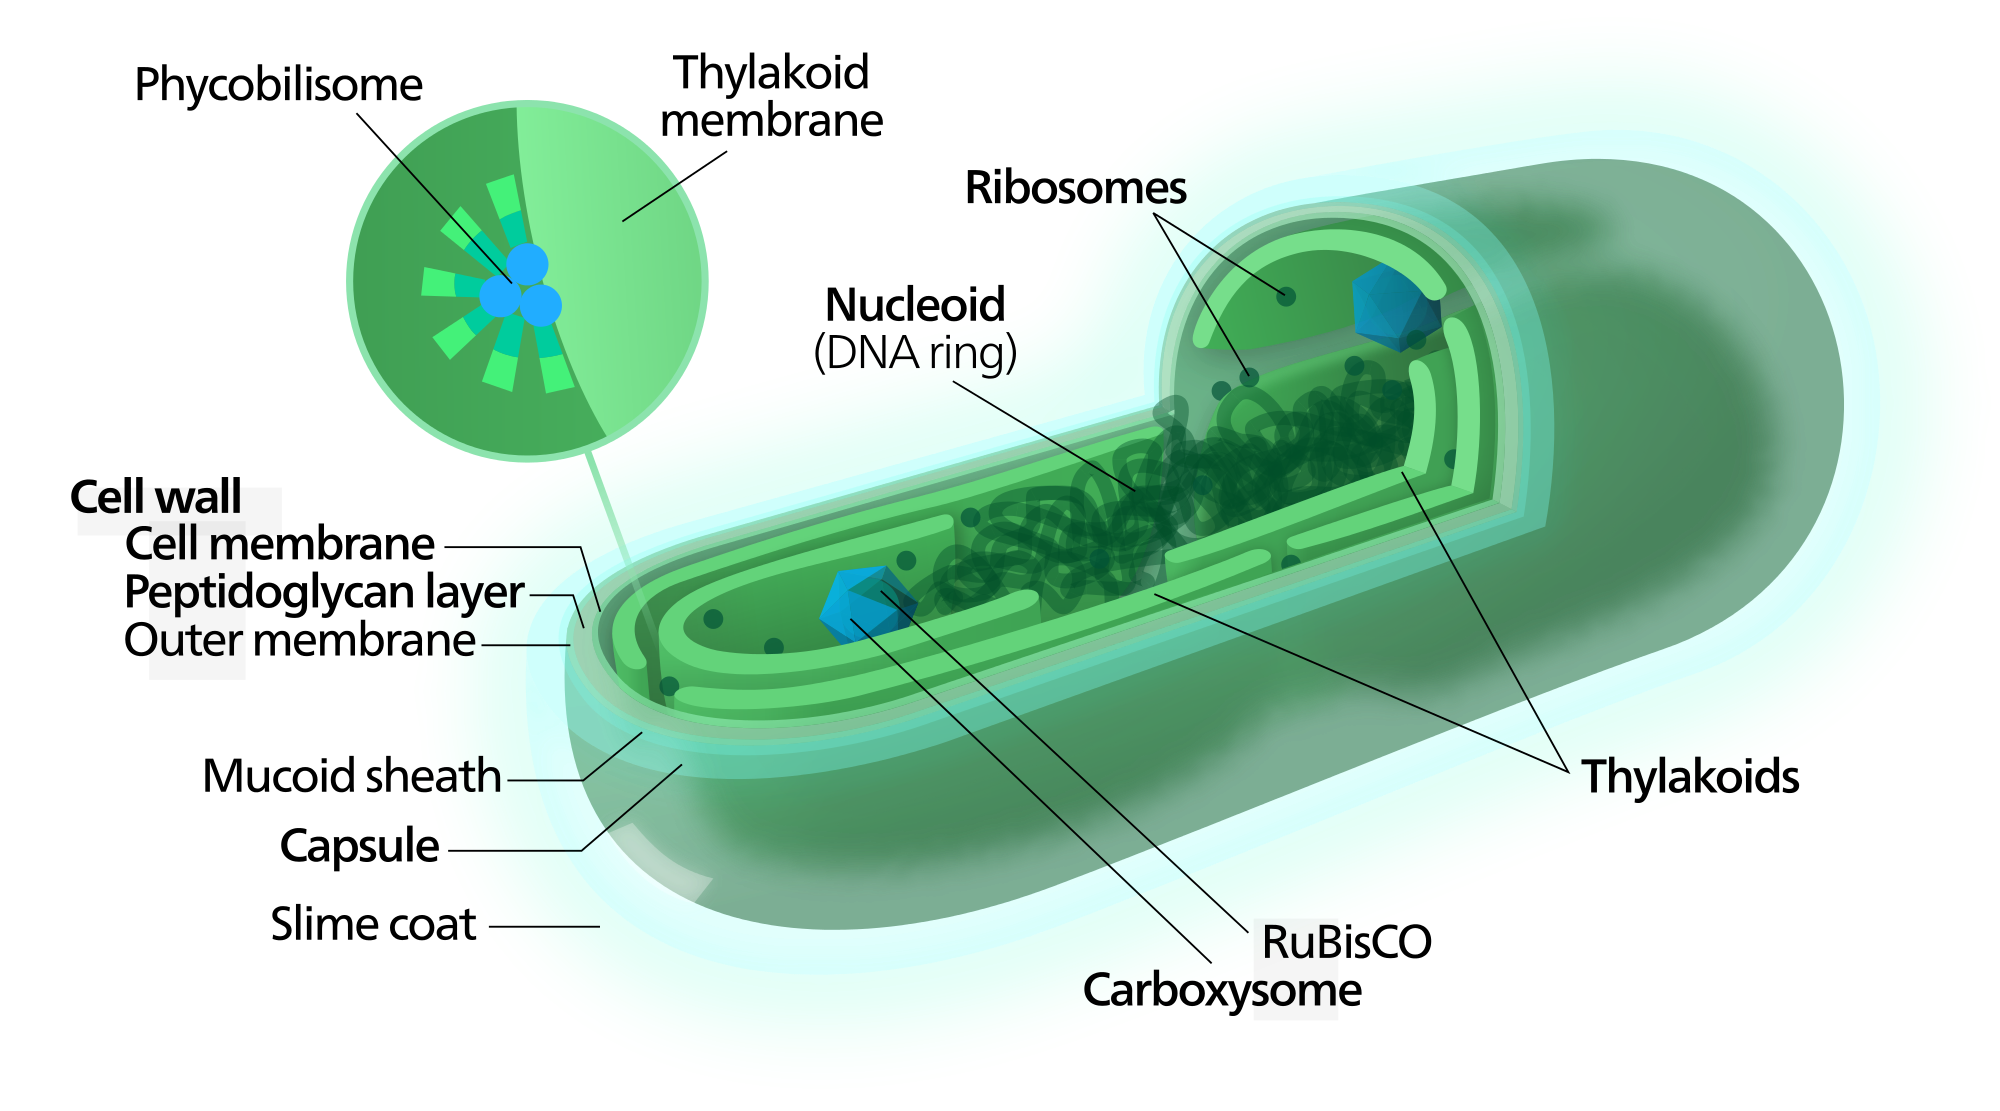
\includegraphics[width=0.8\linewidth]{cyano.png}
\caption{General diagram of cyanobacteria \cite{WikipediaEN:AFM}}
\end{figure}

\end{column} % End of the first column

\begin{column}{\twocolwid} % Begin a column which is two columns wide (column 2)

\begin{columns}[t,totalwidth=\twocolwid] % Split up the two columns wide column again

\begin{column}{\onecolwid} % The first column within column 2 (column 2.1)

%----------------------------------------------------------------------------------------
%	METHODS
%----------------------------------------------------------------------------------------

\begin{figure}
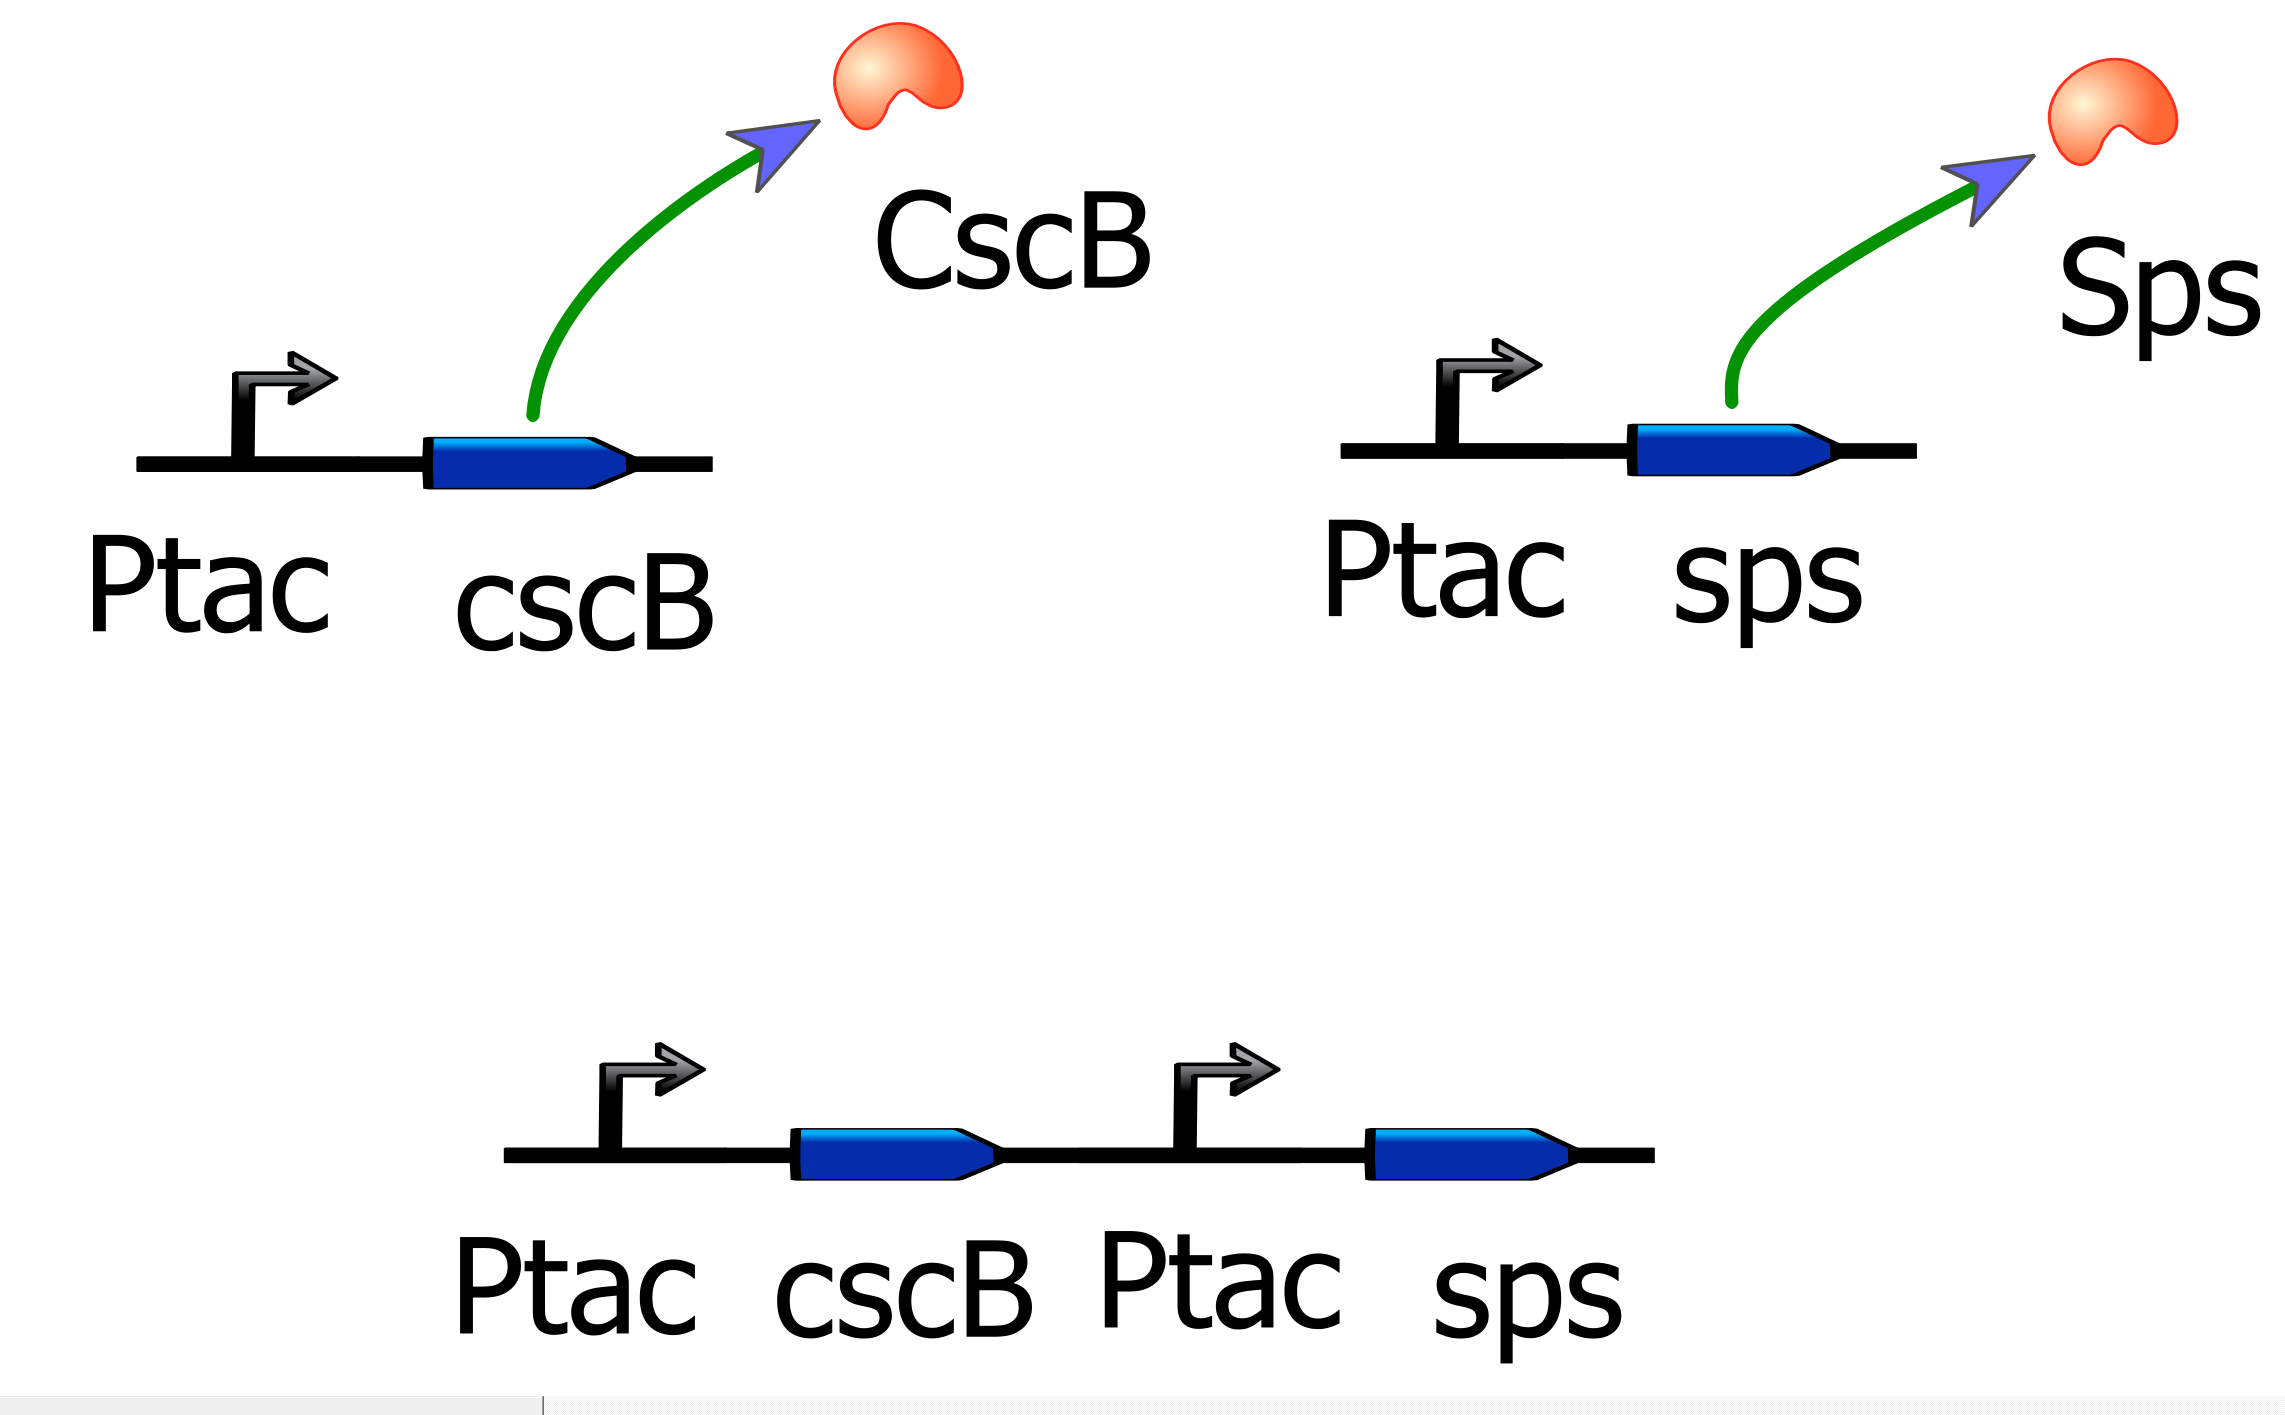
\includegraphics[width=0.8\linewidth]{Q1.PNG}
\caption{Characterizing sucrose production}
\end{figure}

\begin{block}{Methods (Bacteria)}

\begin{itemize}
\item NEB 5-alpha Competent E. coli used in transformation protocols
\item UTEX 2434 \textit{Synechococcus leopoliensis} (very similar to \textit{S. elongatus} PCC 7942) used as model cyanobacteria for testing genetic circuits
\item Transformed cyanobacteria cultured at 35 degrees Celsius and 5\% \ce{CO2} atmosphere on BG-11 agar plates supplemented with sodium bicarbonate
\end{itemize}

\begin{figure}
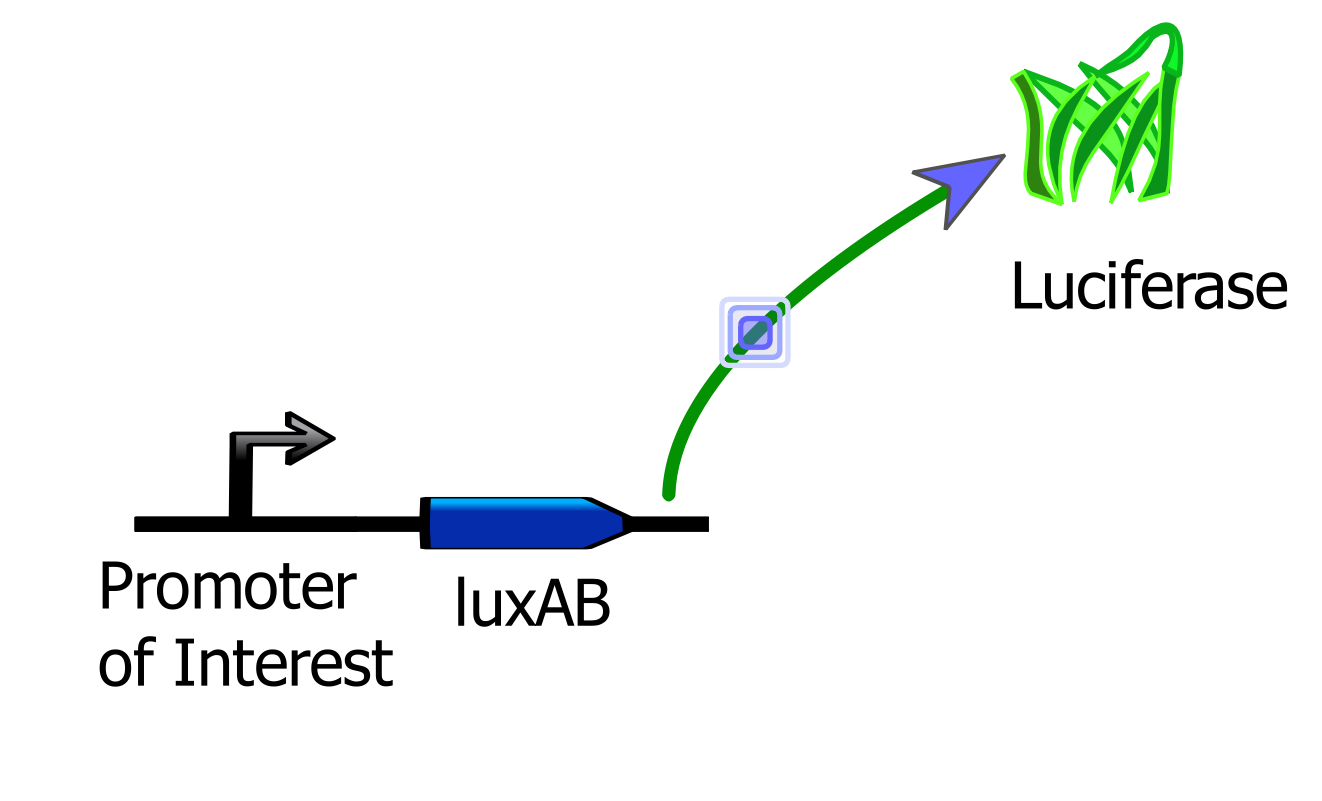
\includegraphics[width=0.8\linewidth]{Q2.PNG}
\caption{Characterizing novel promoters}
\end{figure}

\begin{figure}
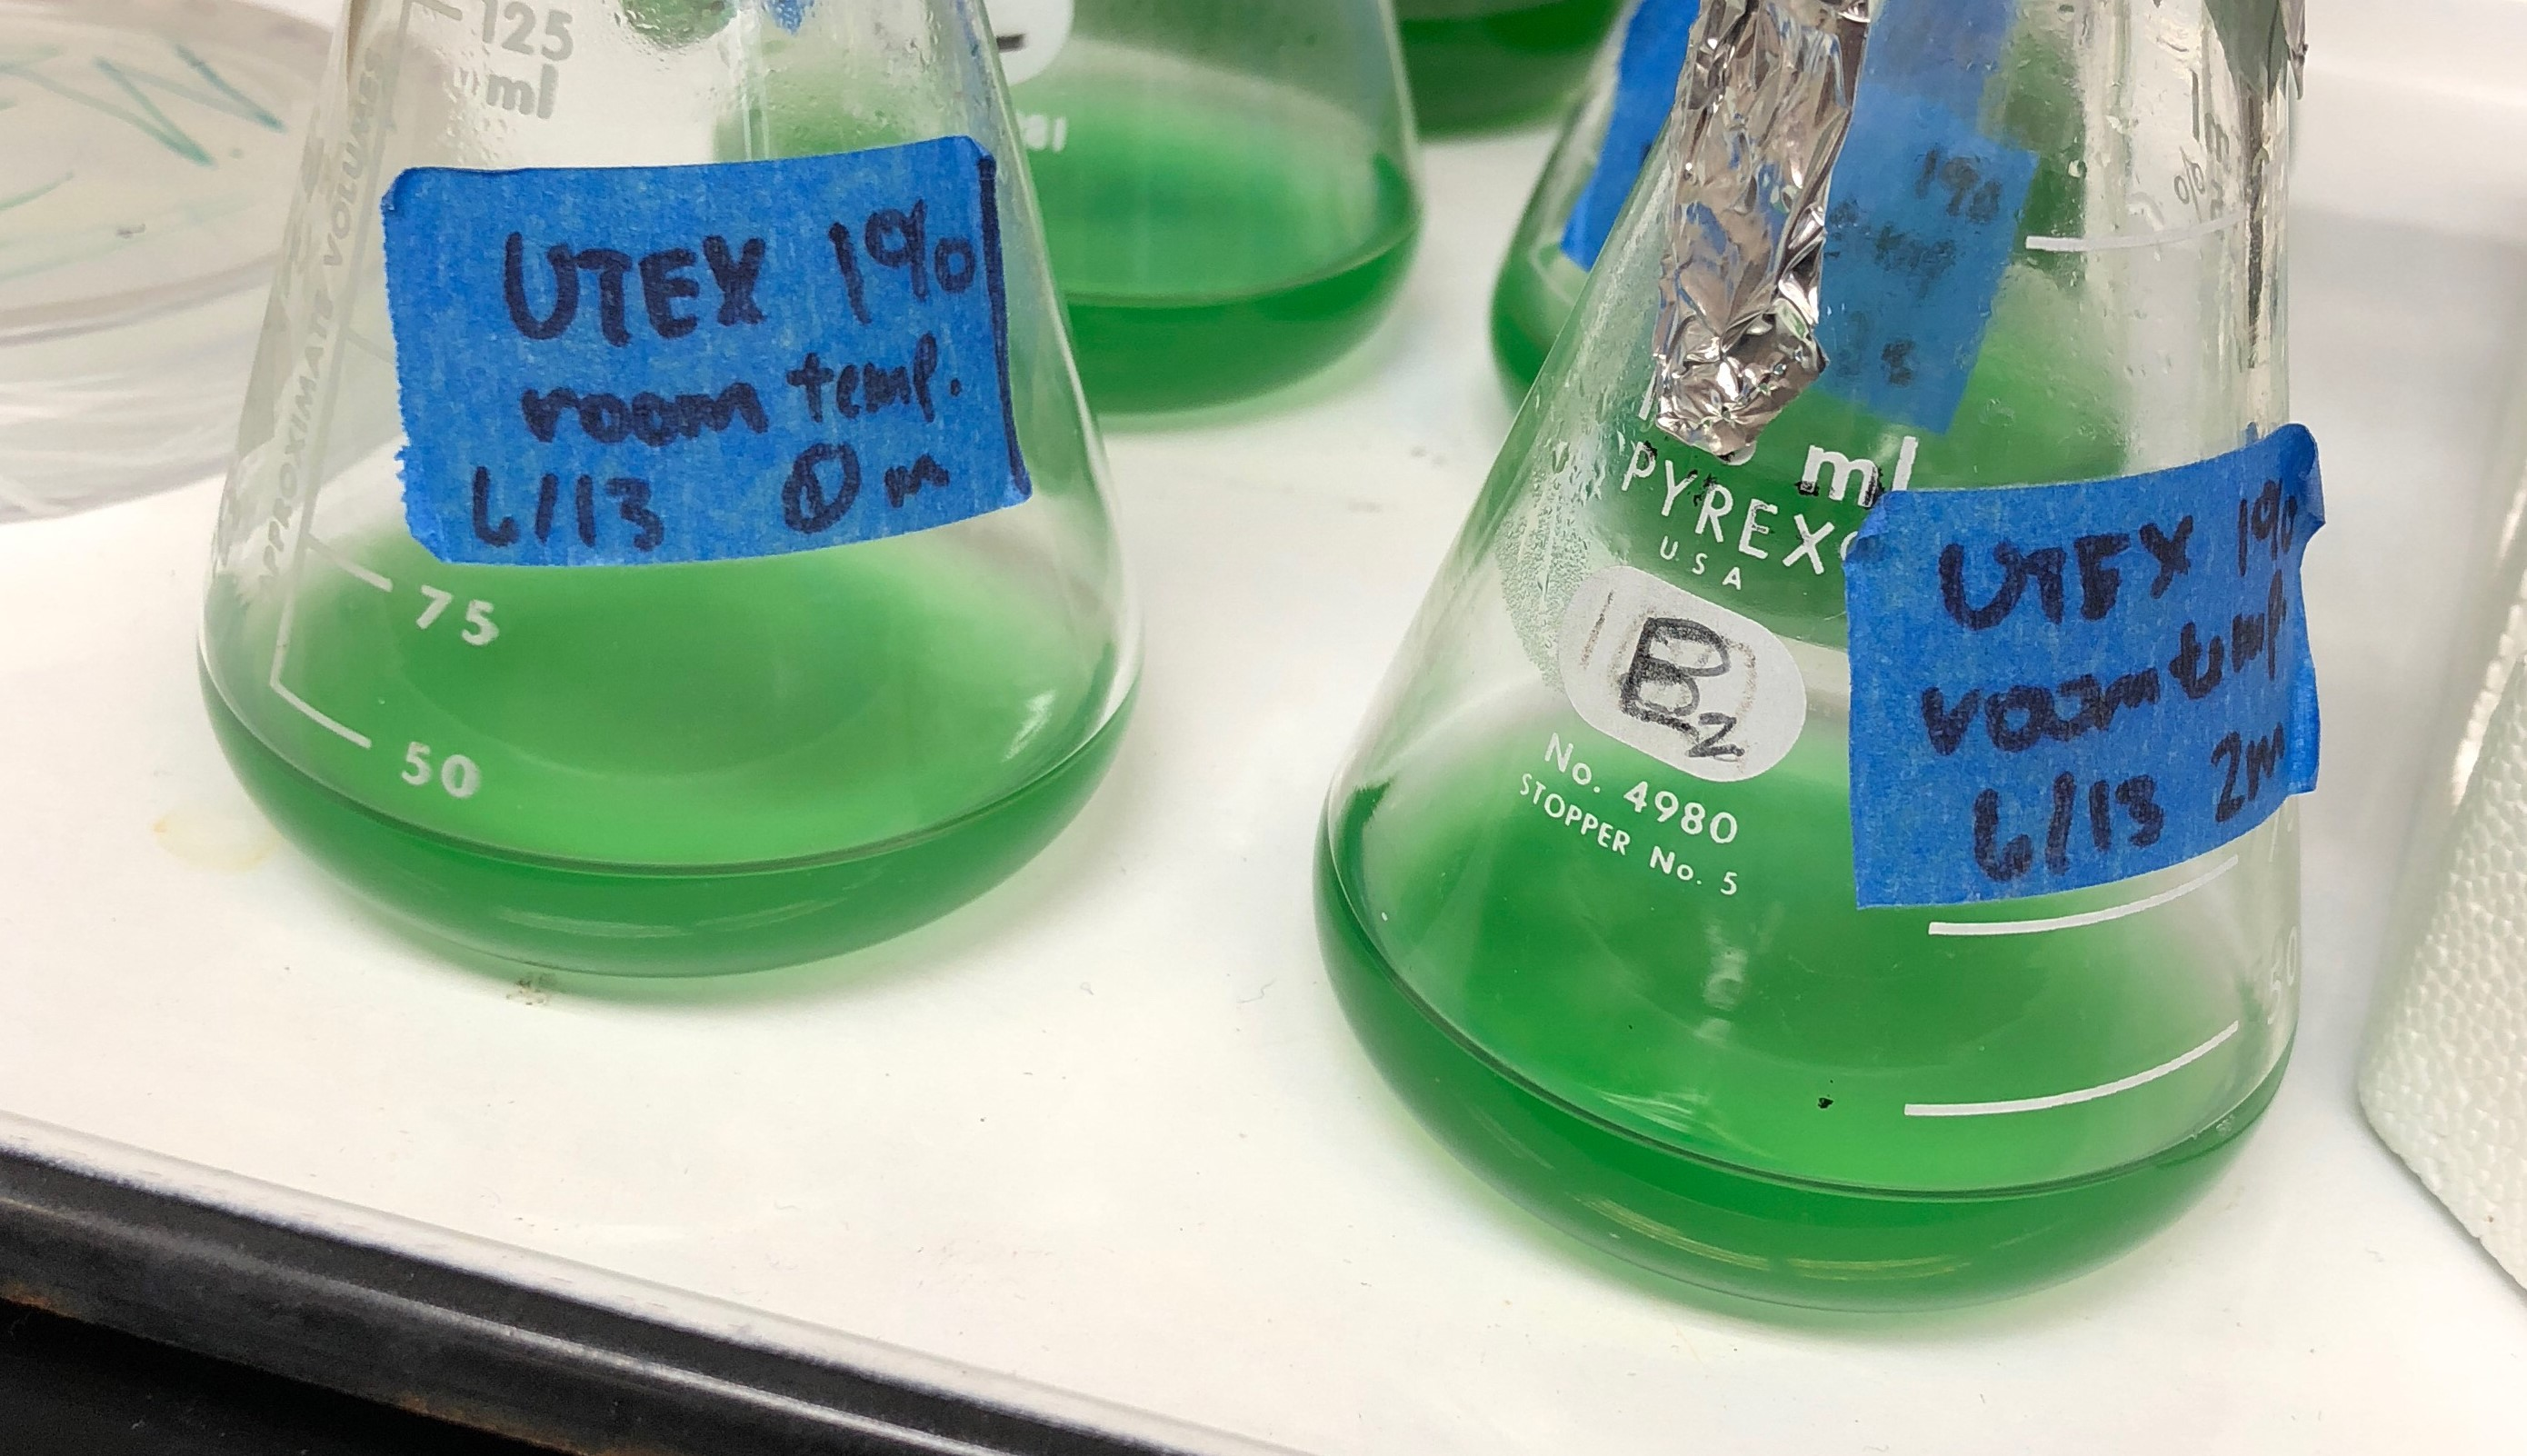
\includegraphics[width=0.8\linewidth]{realcyanos.jpg}
\caption{Liquid cultures of the cyanobacteria}
\end{figure}

\end{block}

\end{column} % End of column 2.1

\begin{column}{\onecolwid} % The second column within column 2 (column 2.2)

\begin{figure}
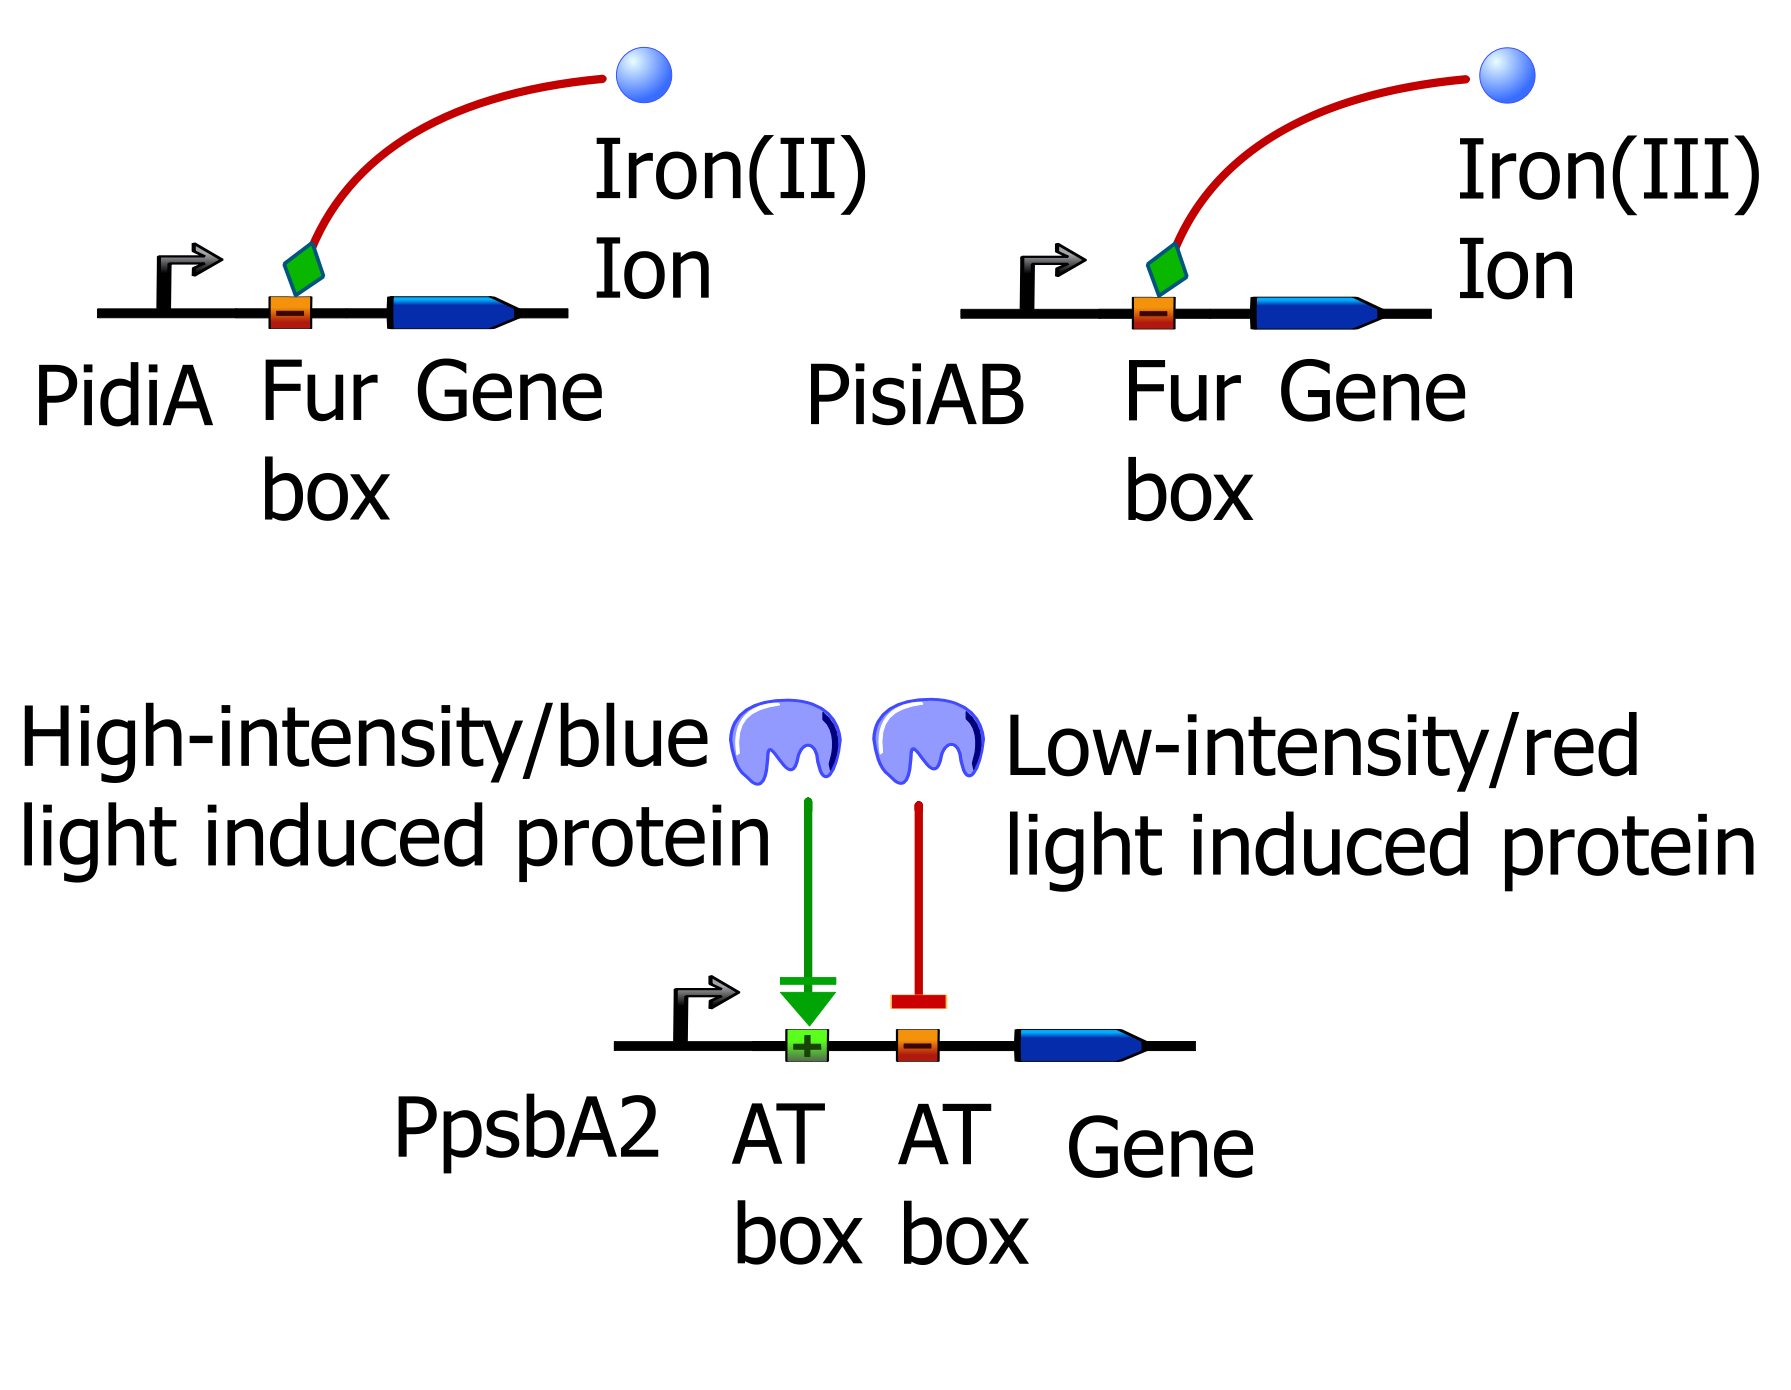
\includegraphics[width=0.8\linewidth]{Q3.PNG}
\caption{Applying novel promoters}
\end{figure}

\begin{block}{Methods (DNA)}

\begin{itemize}
\item Sps and cscB characterized in IPTG-inducible vector pAM2991 from Addgene
\item Novel promoters characterized in luciferase-containing vector pAM1414
\item Final circuits characterized in vector pAM1579
\item Plasmid miniprep from Addgene cultures using Promega PureYield Plasmid Miniprep System
\item PCR of constructs performed using Thermo Scientific Phire Hot Start II Polymerase and purified using Monarch PCR \& DNA Cleanup
\item Genes and promoters of interest inserted into backbone vectors using NEB HiFi Assembly Master Mix, with overlap regions for Gibson assembly designed in the original constructs
\end{itemize}

\vspace{80pt}

\begin{center}

\includegraphics[width=0.6\linewidth]{sbu_logo.jpg}
\end{center}

\end{block}

\end{column} % End of column 2.2

\end{columns} % End of the split of column 2

\end{column} % End of the second column

\begin{column}{\sepwid}\end{column} % Empty spacer column

\begin{column}{\onecolwid} % The third column

%----------------------------------------------------------------------------------------
%	CONCLUSION
%----------------------------------------------------------------------------------------

\begin{block}{Conclusion}
The project is still in progress. We are currently transforming our bacteria, and will be collecting data very soon!
\end{block}

%----------------------------------------------------------------------------------------
%	REFERENCES
%----------------------------------------------------------------------------------------

\begin{block}{References}

\nocite{*} % Insert publications even if they are not cited in the poster
\small{\bibliographystyle{unsrt}
\bibliography{sample}\vspace{0.75in}}

\end{block}

%----------------------------------------------------------------------------------------
%	ACKNOWLEDGEMENTS
%----------------------------------------------------------------------------------------

\setbeamercolor{block title}{fg=red,bg=white} % Change the block title color

\begin{block}{Acknowledgements}

\small{\rmfamily{Stony Brook Undergraduate Biology for providing access to resources such as money, laboratory space, and equipment

Faculty advisors Dr. J. Peter Gergen, Dr. Jarrod French, Dr. Gabor Balazsi, Dr. Steven Glynn, and Dr. Joshua Rest for general project and laboratory advice

Dr. Jackie Collier for advice on cyanobacteria culturing and experimentation

Snapgene for free product licenses

Opentrons for donating the OT-2 robot and accessory parts

GenScript for \$2000 worth of free product and free \$2000

UTEX Culture Collection of Algae for donating cyanobacteria and culture medium

Integrated DNA Technology, Inc., for free gene synthesis

Promega Corporation for \$2000 worth of free product
}} 

\end{block}

%----------------------------------------------------------------------------------------
%	CONTACT INFORMATION
%----------------------------------------------------------------------------------------

\setbeamercolor{block alerted title}{fg=black,bg=norange} % Change the alert block title colors
\setbeamercolor{block alerted body}{fg=black,bg=white} % Change the alert block body colors

\begin{center}
\begin{tabular}{ccc}

\includegraphics[width=0.8\linewidth]{pseg_logo.jpg}
\end{tabular}
\end{center}

\end{column} % End of the third column

\end{columns} % End of all the columns in the poster

\end{frame} % End of the enclosing frame

\end{document}
